    \documentclass[12pt,
        usenames, % allows access to some tikz colors
        dvipsnames % more colors: https://en.wikibooks.org/wiki/LaTeX/Colors
    ]{article}
    \usepackage{
        amsmath,
        amssymb,
        times,
        fancyhdr, % page styling
        lastpage, % footer fanciness
        hyperref, % various links
        setspace, % line spacing
        amsthm, % newtheorem and proof environment
        mathtools, % \Aboxed for boxing inside aligns, among others
        float, % Allow [H] figure env alignment
        enumerate, % Allow custom enumerate numbering
        graphicx, % allow includegraphics with more filetypes
        wasysym, % \smiley!
        upgreek, % \upmu for \mum macro
        listings, % writing TrueType fonts and including code prettily
        tikz, % drawing things
        booktabs, % \bottomrule instead of hline apparently
        cancel % can cancel things out!
    }
    \usepackage[margin=1in]{geometry} % page geometry
    \usepackage[
        labelfont=bf, % caption names are labeled in bold
        font=scriptsize % smaller font for captions
    ]{caption}
    \usepackage[font=scriptsize]{subcaption} % subfigures

    \newcommand*{\scinot}[2]{#1\times10^{#2}}
    \newcommand*{\dotp}[2]{\left<#1\,\middle|\,#2\right>}
    \newcommand*{\rd}[2]{\frac{\mathrm{d}#1}{\mathrm{d}#2}}
    \newcommand*{\pd}[2]{\frac{\partial#1}{\partial#2}}
    \newcommand*{\rtd}[2]{\frac{\mathrm{d}^2#1}{\mathrm{d}#2^2}}
    \newcommand*{\ptd}[2]{\frac{\partial^2 #1}{\partial#2^2}}
    \newcommand*{\md}[2]{\frac{\mathrm{D}#1}{\mathrm{D}#2}}
    \newcommand*{\pvec}[1]{\vec{#1}^{\,\prime}}
    \newcommand*{\svec}[1]{\vec{#1}\;\!}
    \newcommand*{\bm}[1]{\boldsymbol{\mathbf{#1}}}
    \newcommand*{\ang}[0]{\;\text{\AA}}
    \newcommand*{\mum}[0]{\;\upmu \mathrm{m}}
    \newcommand*{\at}[1]{\left.#1\right|}

    \newtheorem{theorem}{Theorem}[section]

    \let\Re\undefined
    \let\Im\undefined
    \DeclareMathOperator{\Res}{Res}
    \DeclareMathOperator{\Re}{Re}
    \DeclareMathOperator{\Im}{Im}
    \DeclareMathOperator{\Log}{Log}
    \DeclareMathOperator{\Arg}{Arg}
    \DeclareMathOperator{\Tr}{Tr}
    \DeclareMathOperator{\E}{E}
    \DeclareMathOperator{\Var}{Var}
    \DeclareMathOperator*{\argmin}{argmin}
    \DeclareMathOperator*{\argmax}{argmax}
    \DeclareMathOperator{\sgn}{sgn}
    \DeclareMathOperator{\diag}{diag\;}

    \DeclarePairedDelimiter\bra{\langle}{\rvert}
    \DeclarePairedDelimiter\ket{\lvert}{\rangle}
    \DeclarePairedDelimiter\abs{\lvert}{\rvert}
    \DeclarePairedDelimiter\ev{\langle}{\rangle}
    \DeclarePairedDelimiter\p{\lparen}{\rparen}
    \DeclarePairedDelimiter\s{\lbrack}{\rbrack}
    \DeclarePairedDelimiter\z{\lbrace}{\rbrace}

    % \everymath{\displaystyle} % biggify limits of inline sums and integrals
    \tikzstyle{circ} % usage: \node[circ, placement] (label) {text};
        = [draw, circle, fill=white, node distance=3cm, minimum height=2em]
    \definecolor{commentgreen}{rgb}{0,0.6,0}
    \lstset{
        basicstyle=\ttfamily\footnotesize,
        frame=single,
        numbers=left,
        showstringspaces=false,
        keywordstyle=\color{blue},
        stringstyle=\color{purple},
        commentstyle=\color{commentgreen},
        morecomment=[l][\color{magenta}]{\#}
    }
    \usepackage[
        backend=bibtex8,
        style=nature]{biblatex}
\defbibenvironment{bibliography}
  {\noindent}
  {\unspace}
  {\printtext[labelnumberwidth]{%
     \printfield{labelprefix}%
     \printfield{labelnumber}}%
   \addspace}
\renewbibmacro*{finentry}{\finentry\addspace}
\bibliography{Su_FINESST_2019}
\AtEveryBibitem{\clearfield{title}}
\begin{document}

\def\Snospace~{\S{}} % hack to remove the space left after autorefs
\renewcommand*{\sectionautorefname}{\Snospace}
\renewcommand*{\appendixautorefname}{\Snospace}
\renewcommand*{\figureautorefname}{Fig.}
\renewcommand*{\equationautorefname}{Eq.}
\renewcommand*{\tableautorefname}{Tab.}

\singlespacing

\pagestyle{fancy}
\rfoot{Yubo Su}
\rhead{}
\cfoot{\thepage/\pageref{LastPage}}

\title{Nonlinear Tidal Dissipation in Binary White Dwarfs}
\author{Yubo Su}
\date{}

\maketitle

\section{Background and Proposed Research}

\subsection{White Dwarf Binaries}

Compact white dwarf (WD) binary systems, with orbital periods in the range of
minutes to hours, are important for a range of astrophysical problems. They are
the most important sources of gravitational waves (GWs) for the Laser
Interferometric Space Antenna (LISA)\cite{lisa}. They are also thought to
produce interesting optical transients such as tidal novae\cite{tidal_novae},
underluminous supernovae\cite{underlum}, and Ca-rich fast
transients\cite{carich}. Most importantly, they have been proposed as the likely
progenitors of type Ia supernovae (e.g.~\cite{Ia0,webbink} or more
recently\cite{Ia1,Ia2}). While presently only a few tens of compact WD binaries
are known\cite{lsst_wd}, \emph{Gaia} (currently gathering data) is expected to
expand the catalog to a few hundred\cite{lsst_wd} (results based on
\emph{Gaia}'s second data release have already begun to
appear\cite{gaiaDD,gaiaDD2}), and the Large Synoptic Survey Telescope (LSST,
first light scheduled for 2020) will likely detect a few thousand
more\cite{lsst_wd}. These observations will significantly advance the
understanding of WD binaries. My proposed theoretical and computational research
is well-timed to take advantage of these new advances.

In spite of the broad importance of WD binaries, the evolution of these systems
prior to their final merger is not well understood. Much of this uncertainty
comes from our imprecise understanding of tidal interactions, which play an
important role during a compact WD binary's inspiral\cite{fullerII}. Studies
show that these interactions manifest as tidal excitation of internal gravity
waves (IGW), waves in the WD fluid restored by the buoyancy force due to density
stratification\cite{fullerI}. As these waves propagate outwards towards the
surface, they grow in amplitude until they break, as do ocean waves on a shore,
and transfer both energy and angular momentum from the binary orbit to the outer
envelope of the WD\cite{fullerI,fullerII}.

Previous works have found that this tidal dissipation mechanism can generate
significantly more energy than thermal radiation from the WD surface alone and
is thus a major contributor to the WD energy budget\cite{fullerII,fullerIV}.
However, these works parameterized the wave breaking process without
hydrodynamical simulations. The details of tidal dissipation, namely the
location and spatial extent of the wave breaking, affect the observable outcome:
dissipation near the surface of the WD can be efficiently radiated away and
simply brightens the WD, while dissipation deep in the WD causes an energy
buildup that results in energetic flares\cite{tidal_novae}. Similar works in
other fields find that numerical simulations capturing the strongly nonlinear
wave breaking process find new behavior that cannot be described by linear and
weakly nonlinear theory\cite{winters1994,barker_ogilvie}. Such fully nonlinear
numerical simulations have not been performed for WDs.

\subsection{Proposed Research}

Characterizing the location and spatial extent of tidal dissipation in WD
binaries will require numerical simulation to capture the turbulent cascade to
small scales causing wave breaking. \textbf{I propose to study the dynamical
effects of tidal dissipation via nonlinear IGW breaking in binary WDs.} To
accomplish this, I aim to address the following three aims:
\begin{itemize}
    \item Characterize the location, spatial extent, and other properties of
        wave breaking in realistic WD models via direct numerical simulation.
        The location and spatial extent will furnish a simple yet effective
        parameterization of tidal dissipation. \autoref{s:2} describes the
        steps required for this aim.

    \item Predict signatures of tidal dissipation over a wide range of possible
        WD systems. In particular, I will describe the impact of tidal heating
        on the apparent temperature of a binary WD and maybe even the production
        of observable flares. \autoref{s:3} details my plan to do so.

    \item Compute modified GW templates for LISA that account for changes in the
        phase evolution of the orbit due to tidal dissipation. \autoref{s:4}
        elaborates on how I will perform this computation.
\end{itemize}

\section{Nonlinear Tidal Dissipation}\label{s:2}

\subsection{Background and Preliminary Work}

The current understanding of tidal synchronization in WD binaries is laid out
in~\cite{fullerII}: a tidally-excited train of IGW undergoes wave breaking in
the outer envelope of the WD, locally depositing angular momentum and
synchronizing the WD spin to the binary orbit. A similar process may also
operate in stellar binaries consisting of early type stars\cite{zahn75,gn89},
the only major difference being in the specifics of wave
excitation\footnote{While IGWs in stars are excited at their
radiative-convective boundaries, IGWs in WDs are excited at sharp changes in
composition.}. Nevertheless, direct numerical simulation of the wave breaking
process has not been performed in either of these systems. Since wave breaking
is a strongly nonlinear phenomenon, where a larger wave breaks down into many
smaller-scale waves, numerical simulation is paramount to an accurate
understanding of IGW breaking.

IGW breaking has been studied in detail in atmospheric sciences. The wave
breaking process proceeds as follows: initially, as the IGW reaches nonlinear
amplitudes, it breaks down via the parametric subharmonic instability and
transfers energy and angular momentum from the wave to the mean flow of the
fluid\cite{drazin}. Subsequently, after the mean flow velocity reaches the
horizontal phase velocity of the IGW, a critical layer through which the IGW
cannot propagate forms. A well-known calculation shows that the IGW is nearly
completely absorbed at this critical layer in the linear approximation and
endows the atmosphere with a mean horizontal flow\cite{booker_bretherton,hazel}.
However, when this mean flow absorption was numerically studied including full
nonlinear interactions, new phenomena not described by the linear theory
(reflection off the critical layer and sharpening of the mean flow) were
observed\cite{jones_num,winters1994} that affected the evolution of the
atmosphere over time. \emph{This highlights the importance of numerical
simulation in capturing the wave breaking process.}

To gain insight into the tidal dissipation process, I began by using the
spectral hydrodynamics code Dedalus\cite{dedalus} to study IGW breaking in a 2D
isothermal, stratified atmosphere. A spectral code like Dedalus is ideal for
simulating complex hydrodynamical phenomena, as spectral methods have no
inherent numerical viscosity and so better resolve the nonlinear cascade to
small length scales in wave breaking.

Working with Dr.\ Daniel Lecoanet (Princeton; one of the authors of the Dedalus
code) and my advisor, Prof.\ Dong Lai, I simulated an upward-propagating IGW
wavetrain excited at the bottom of the atmosphere. I observe the excited wave
breaking and depositing horizontal momentum in the fluid, causing the fluid to
acquire an average horizontal flow, consistent with previous
studies\cite{fullerII}. I derive simple formulae for the location and spatial
extent of the dissipation zone where the IGW is absorbed by the fluid. More
interestingly, I observe partial reflection of the IGW at the synchronization
layer\cite{me}, a phenomenon not considered in the current astrophysical
literature but consistent with the aforementioned results\cite{winters1994}. A
sample simulation is presented in \autoref{fig:nl_fluxes}. I am preparing these
results for publication\cite{me}.

\begin{figure}[!h]
    \centering
    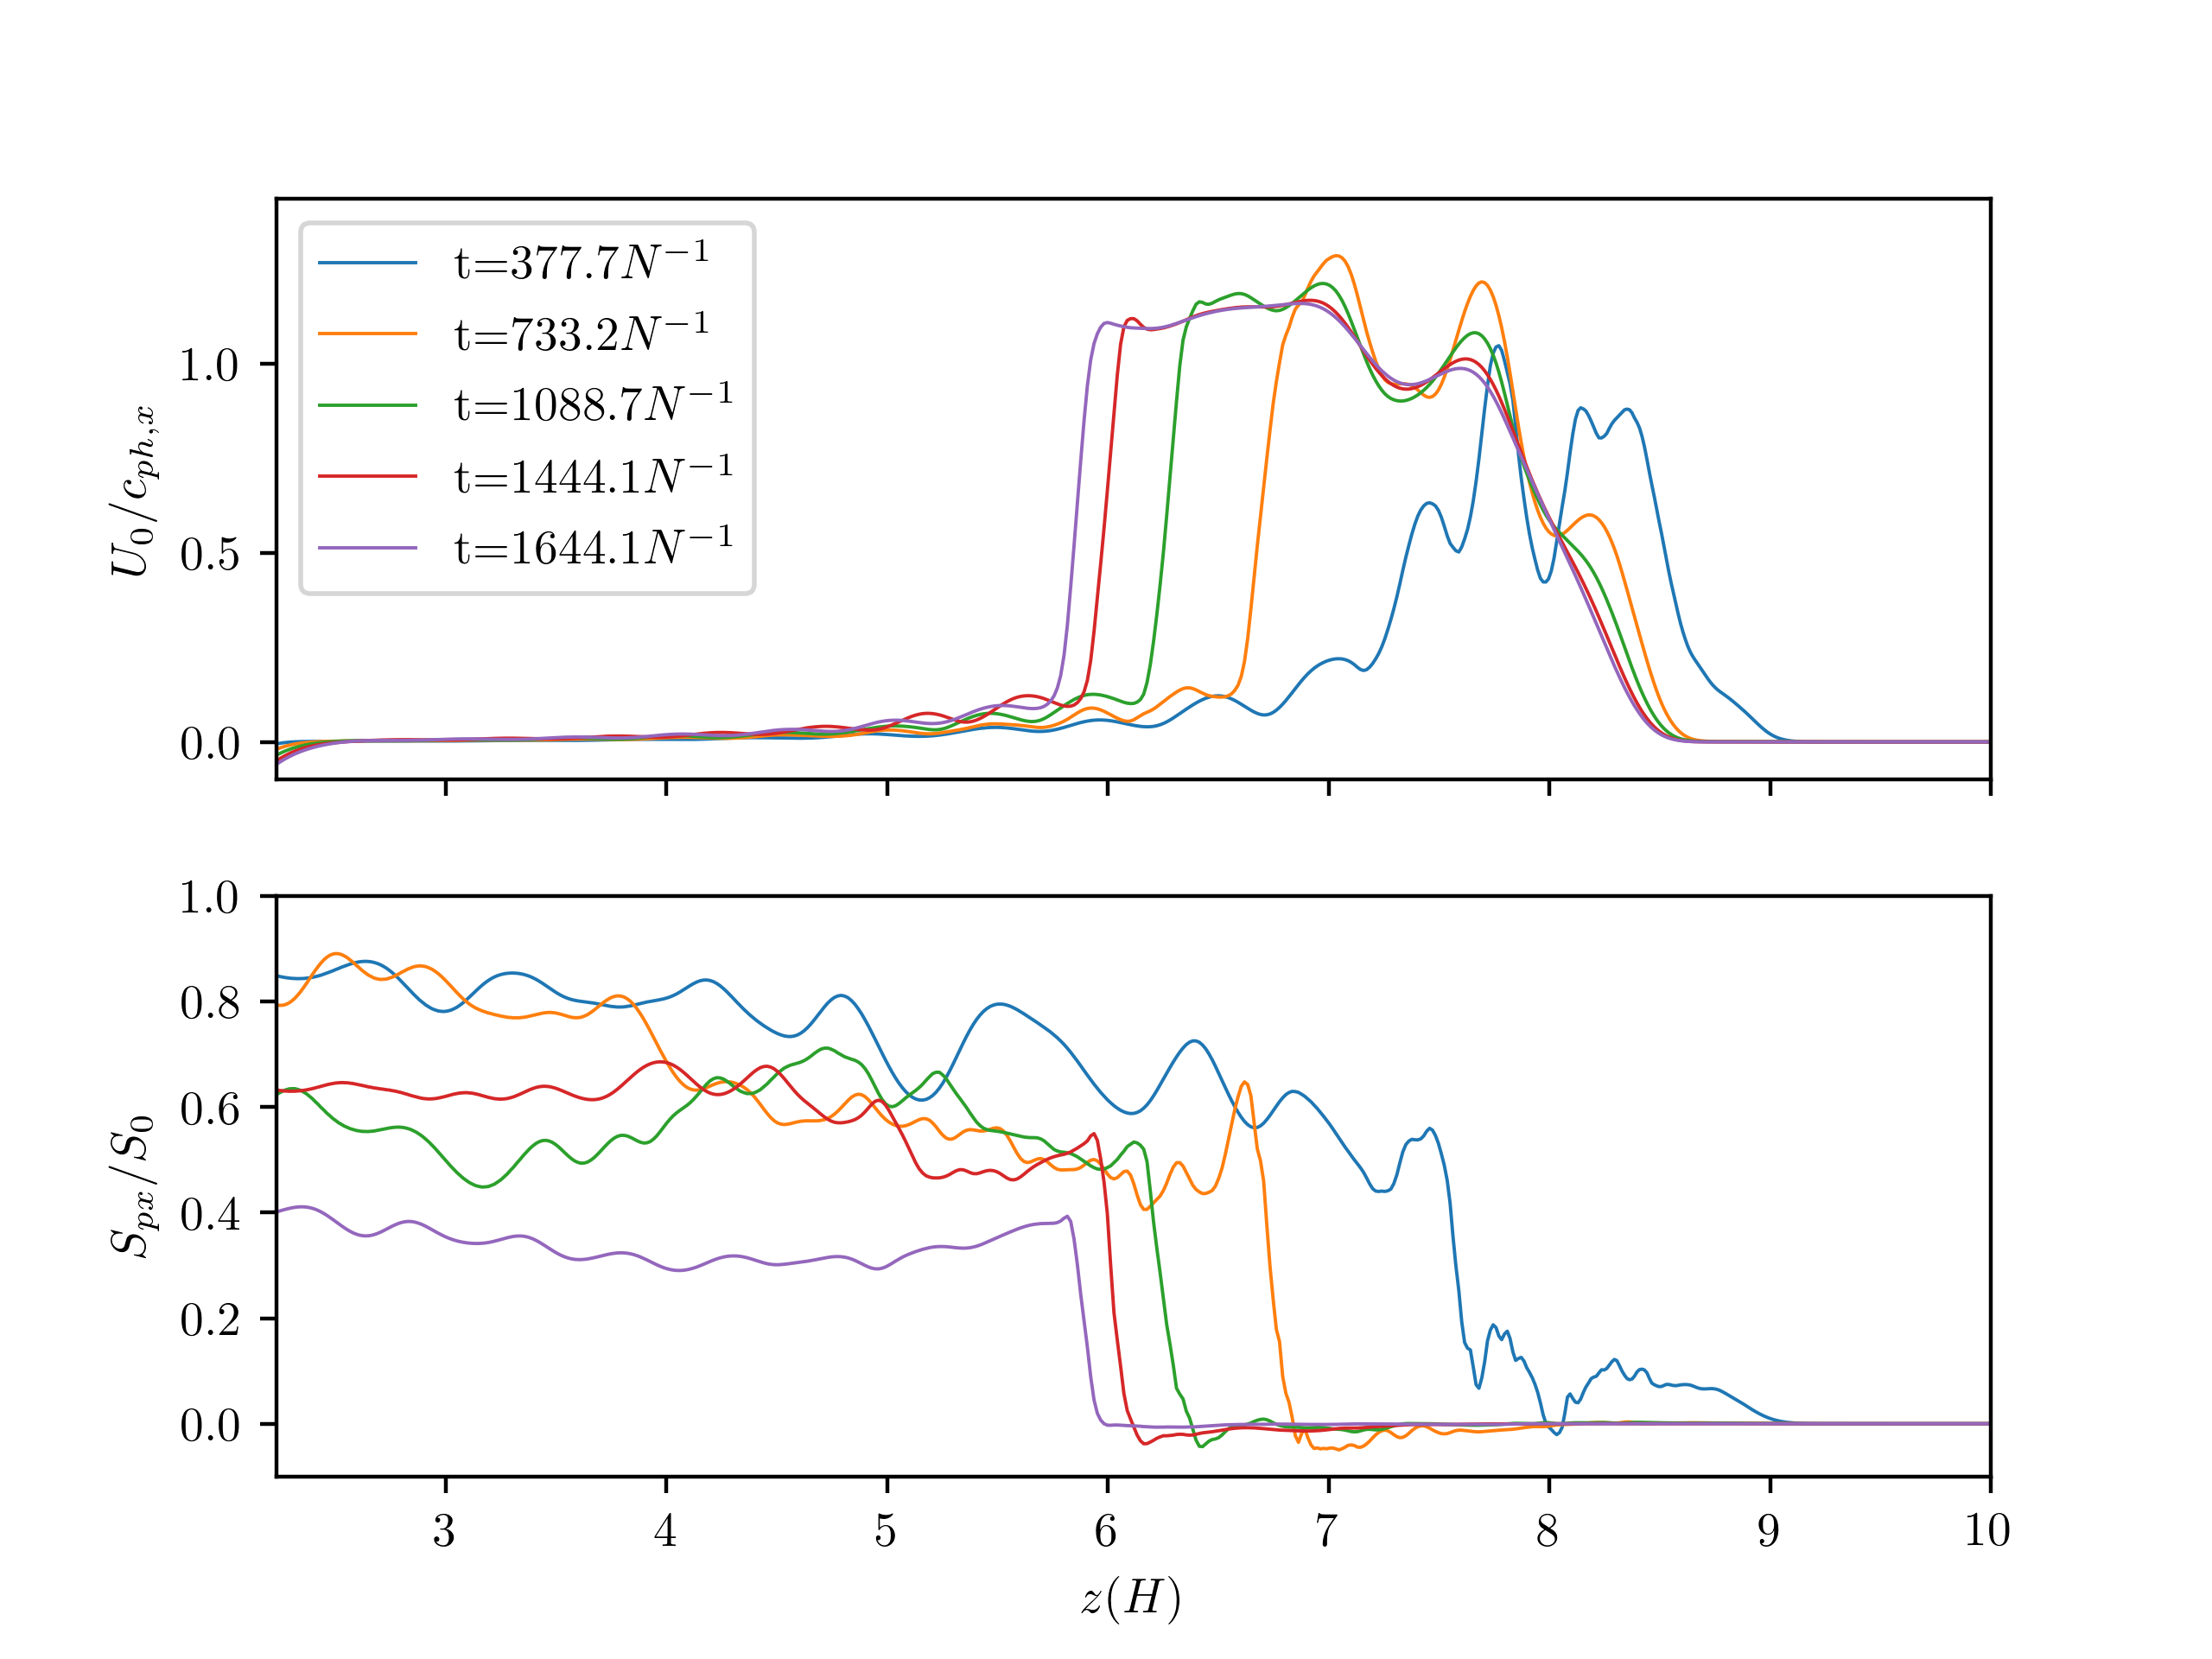
\includegraphics[width=0.7\textwidth]{nl_fluxes.png}
    \caption{The evolution of the average horizontal flow velocity of the fluid
    $U_0$ (in units of $c_{ph,x}$ the horizontal phase velocity of the IGW) and
    horizontal momentum flux contained in the IGW $S_{px}(z)$ (in units of the
    total excited flux $S_0$) for one of my simulations. Different colored lines
    correspond to different times in the simulation. Times are measured in units
    of $N^{-1}$, the inverse of the Brunt-V\"ais\"al\"a frequency (or the
    buoyancy period), and heights in units of $H$ the scale height of the
    density stratification. IGW are excited at $z = 2H$ and propagate to higher
    $z$ before undergoing wave breaking. The sharp decrease in $S_{px}$ is
    the location of the critical layer where the IGW breaks and drives $U_0$
    towards $c_{ph, x}$; it moves to lower $z$ over time. The apparent decrease
    in $S_{px}$ at later times indicates reflection off the critical
    layer.}\label{fig:nl_fluxes}
\end{figure}

\subsection{Proposed Work}

It is therefore clear that full numerical modeling of IGW breaking is necessary
to fully characterize tidal dissipation. The first aim of my proposal is then:
\textbf{I will extend my preliminary results to characterize the dynamics of
nonlinear IGW breaking in realistic WDs.} Via numerical simulation, I will
develop simple models for tidal dissipation that can be used to study WD
evolution under tidal heating without performing further simulations. I will
continue my work in the following stages:
\begin{itemize}
    \item I will perform simulations examining the validity of my results in
        more realistic geometries, including polar and spherical geometries. I
        will continue to use Dedalus, which also supports these coordinate
        systems.

    \item I will extend my simulations to realistic WD models and equations of
        state such as those in~\cite{brassard1992}, continuing to track the
        location and spatial extent of the dissipation layer as well as any new
        phenomena. As WDs vary widely in composition and effective temperature,
        studying representative WD models is vital to obtaining a robust
        characterization of tidal dissipation. My selected WD models are those
        used in the current literature\cite{fullerII, fullerIV}.
\end{itemize}

\section{Tidal Heating Thermodynamics}\label{s:3}

\subsection{Background}

As discussed earlier, compact WD binaries exhibit a range of observed and
hypothesized optical transients. Tidal novae\cite{tidal_novae}, underluminous
supernovae\cite{underlum}, and Ca-rich fast transients\cite{carich} are all
hypothesized to arise in WD binary systems. Given that tidal heating can become
a significant contributor to a WD's total energy budget, a realistic model of
tidal dissipation is important to understanding a binary WD's thermodynamic
evolution during inspiral.

In~\cite{tidal_novae} (hereafter FL), the authors use MESA to study the
production of tidal novae in binary WDs. A simple two-zone parameterization
where the tidal heat is deposited throughout the outer zone was used to model
tidal dissipation. They find that cool WDs in sufficiently compact binaries
(orbital period $\lesssim 15$ minutes) may incur a thermonuclear detonation of
the hydrogen envelope. WD binaries with such short orbital periods have been
observed, e.g.\ SDSS J065133+284423 has a period of 12.75 minutes\cite{12min}.
FL fits the observed properties of SDSS J065133+284423 to their tidal heating
models and finds evidence for tidal heating of the secondary WD in SDSS
J065133+284423. From their fits, FL are able to estimate the temperature of the
WD in the absence of tidal heating. As WDs form around a well known temperature
and cool predictably over time, accounting for tidal heating equates to a large
correction to the age of the WD\@. This illustrates the importance of accurately
modeling tidal interactions when inferring physical properties.

\subsection{Proposed Work}

With the tidal dissipation models I will develop, I will be able to perform a
simulation similar to that in FL but with a more realistic tidal interaction.
The second aim of my proposal is accordingly: \textbf{I will use my tidal
% "obtained in Section 2"
dissipation profiles to simulate a binary WD undergoing tidal heating and make
comparisons to observational data.} The location of the tidal heating is a key
ingredient in determining whether deposited energy can be efficiently transfered
away or whether the WD experiences sudden detonations. As such, an improved
understanding of the properties of tidal dissipation is important to proper
forecasting of binary WDs' thermodynamic evolution. Moreover, while only a few
sufficiently compact WD binaries were available at the time of writing of FL,
\emph{Gaia} data releases 2 and 3 will provide many more compact WD binaries to
examine for evidence of tidal heating.

Using MESA, I will evolve various WD models undergoing tidal heating. From these
simulations, I will extract the increased temperature of the WDs and make
comparisons to observational data, in particular to WDs in new \emph{Gaia} data
releases. I will also identify the occurrence rate and observational properties
of any predicted optical transients such as tidal novae and attempt to identify
them among existing detected events. Predictions of the occurence rates of such
phenomena are vital to guiding future observations. Finally, comparison of
observational data from known WD binaries to simulations could yield new
insights to the behavior of degenerate matter.

\section{Tidal Heating and LISA}\label{s:4}

As discussed earlier, WD binaries are a primary source of GW radiation for
LISA\@. LISA will attain optimal sensitivity at frequencies
$10^{-4}$--$10^{-1}\;\mathrm{Hz}$\cite{LISA_band}. Exactly in this frequency
range, tidal effects act to synchronize the orbit of the WDs to the binary
orbit and transfer energy from the orbit into the WDs. While the decay
of the binary orbit is still mostly driven by GW radiation, the tidal energy
dissipation rate grows to $\sim10^{-2}$ the GW energy
dissipation\cite{fullerII,fullerIV}. An effect of such a magnitude causes the
phase of the emitted GWs to significantly from the point-mass binary
prediction; the emitted wave may exhibit ``missing cycles'' due to tidal
effects\cite{fullerII}. GW astronomy uses matched filtering, where a library of
template waveforms is matched against instrument data, to identify GW signals.
As such, the accuracy and completeness of the template library is of utmost
importance.

The final aim of my proposal is then: \textbf{I will use my tidal dissipation
model to compute WD binary GW waveforms including tidal dissipation for use in
the LISA detection pipeline}. This aim is much less computationally expensive
than it appears: LISA-band WD binaries can be well described using the Newtonian
dynamics of two co-orbiting point masses\cite{DWD_pointmass}. The resultant GW
emission can then be accurately computed using the weak gravity quadrupole
approximation (see e.g.~\cite{peters,lsst_wd}). Under these two approximations,
the GW waveform can be computed analytically without resorting to numerical
relativity simulations at all, an enormous computational savings. Thus, I will
compute GW waveforms accounting for the additional phase evolution due to tidal
dissipation. I will publish my corrected waveforms for use by LISA and the GW
community.

\section{Project Timeline}

During the first year of work and first half of the second year, I will complete
my tidal dissipation model. I anticipate the extension of my 2D plane-parallel
work to more complex geometries will be complete within the first half year,
while the extension to realistic WD models will take up to a year. I expect that
these two results together will produce one peer-reviewed publication in
addition to the one currently in preparation.

During the following year, I will use my tidal dissipation model to perform MESA
simulations of tidally heated WDs and compare to observational data. I expect my
MESA simulations and extracting appropriate observables to take about half a
year. I then intend to spend another half year analyzing observational data for
potential signatures of tidal heating or tidal novae. I expect both of these
phases will produce peer-reviewed publications.

Finally, in the last six months I will compute WD binary GW templates for use by
the LISA community. This work will also produce one peer-reviewed publication.

\section{Relevance to NASA Objectives}

This project is extremely relevant to the NASA Astrophysics research program.
My work directly relates to (i) the interactions of particles under the extreme
conditions found in astrophysical situations, (ii) how complex systems create
and shape the structure and composition of the universe on all scales, and (iii)
the development of new techniques that can be applied to future major missions.

My work will improve understanding of possible energetic phenomena that can
occur in compact object binaries. My results concerning angular momentum
transfer via IGW breaking will be applicable to astrophysical systems beyond WD
binaries, for instance angular momentum transfer in stars\cite{l_trans_rev}. I
will devise new ways of analyzing astrophysically interesting systems in
\emph{Gaia} and LSST\@. Finally, my GW templates will be important for LISA GW
detection efforts.

My work has direct relevance to NASA missions in the detectability of
astrophysical transients related to WD binaries. For instance, tidal novae are
theorized to have a similar observational signature to dwarf novae which have
been observed with Chandra and the Hubble Space Telescope, among others.

\printbibliography

\end{document}
